\section{Software Process Representations} \label{diagrams}

In the following section, we use our notation to depict 

\subsection{Software Development Lifecycle (SDLC)}
Royce first introduced and formalised the SDLC in
\cite{Royce:1987:MDL:41765.41801}.
He was quick to criticise the SDLC as a software development methodology, and pointed out its flaws
and inflexibility to handle software development.
In particular, he noted that its roots were in engineering and other physicals sciences, and the
nature of software meant that it was ineffective and caused much work to be redundantly repeated.\\
\\
This model is commonly known as a ``Waterfall" lifecycle development model, due to the way
activities cascaded in the original model.
We reproduce his diagrams in our own notation as follows.
In Figure \ref{waterfallRoyceOne}, we show our interpretation of Royce's unmodified waterfall model.

\begin{figure}[ht!]
	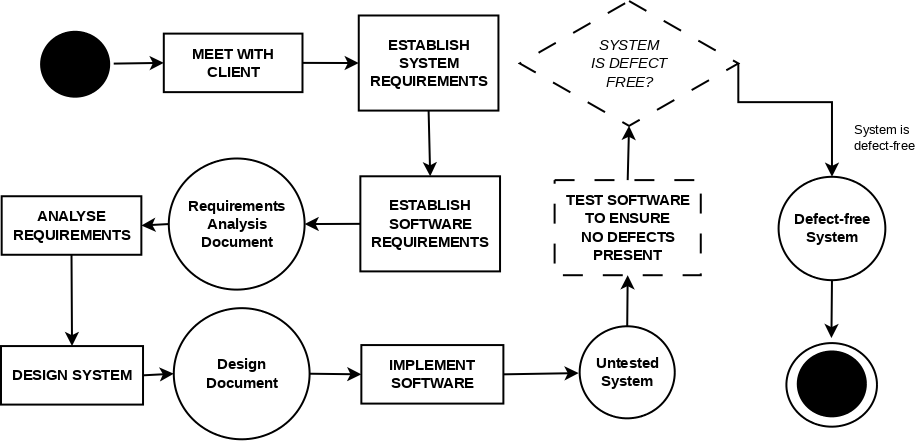
\includegraphics[scale=0.3]{media/WaterfallRoyceOne}
	\caption{Royce's original waterfall model. This is the theoretical way that the SDLC works.}
	\label{waterfallRoyceOne}
\end{figure}

Royce points out the flaws in this model, by revealing that we actually make mistakes and
assumptions when we gather requirements, design a system or implement a system in code.
These assumptions are actually defects that propagate throughout a system, and we are forced to
backtrack to earlier tasks and repeat these tasks in order to fix them.
This can involve backtracking from implementing a feature, to checking how it was designed, to
regathering requirements for this feature upon realising that a client does not actually need that
feature.
Royce claimed this backtracking was quite a significant delay and waste of resources, and we
illustrate his point in our notation in Figure \ref{waterfallRoyceTwo}.

\begin{figure}[ht!]
	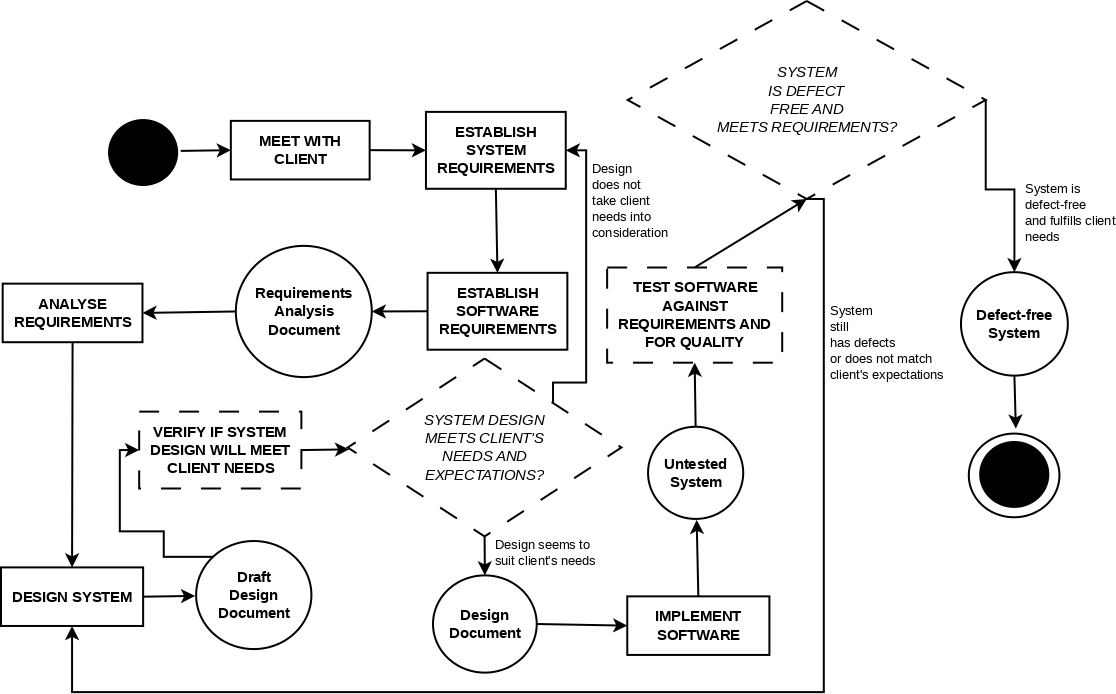
\includegraphics[scale=0.3]{media/WaterfallRoyceTwo}
	\caption{Royce claims that this modified waterfall method was inefficient and caused unnecessary
		backtracking, but that in 1987 it was the current mode of software production.}
	\label{waterfallRoyceTwo}
\end{figure}

Royce suggests an alternative model, which involves iterations and backtracking between stages to
minimise the repeated work.
This recognition that some sort of iteration is necessary to develop good software is perhaps the
beginning of some of the iterative models that we later discuss.
We show Royce's final model in our own notation in \ref{waterfallRoyceThree}, with a heavy emphasis
on verification between each stage to dictate the backtracking.

\pagebreak

\begin{figure}[ht!]
	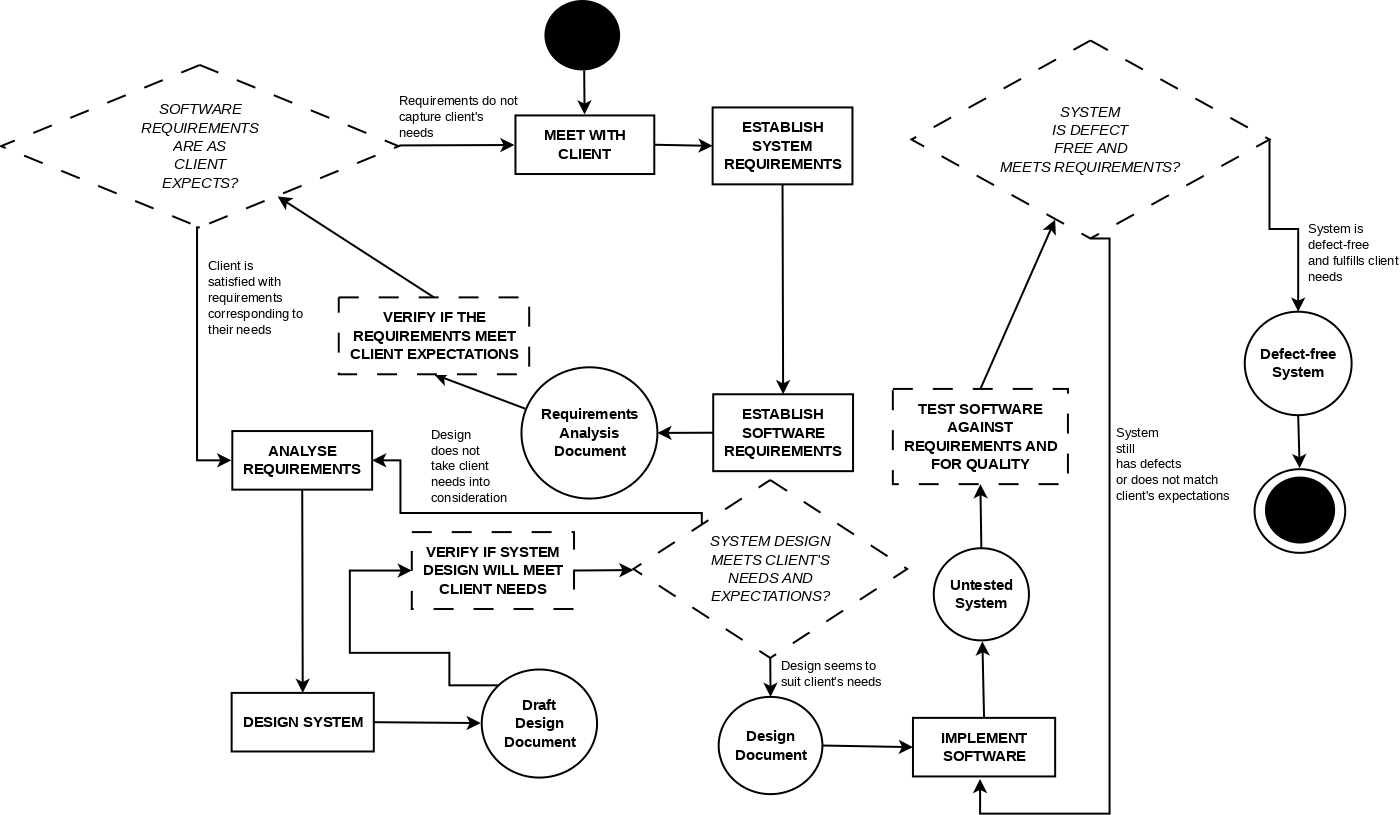
\includegraphics[angle=90,scale=0.3]{media/WaterfallRoyceThree}
	\caption{Royce's final waterfall model resolves the repetition in process work by increasing the
		verification and iteration between stages. We replicate this in our own notation.}
	\label{waterfallRoyceThree}
\end{figure}

\subsection{Spiral}
The Spiral model is introduced by Boehm in \cite{Boehm:1986:SMS:12944.12948}.
It attempts to address some of the weaknesses revealed in SDLC.
It has more concepts of verification and risk analysis built into it.
We show the Spiral model, after it has been unrolled from its original form, in Figure
\ref{Spiral}.\\
\\

\begin{figure}[ht!]
	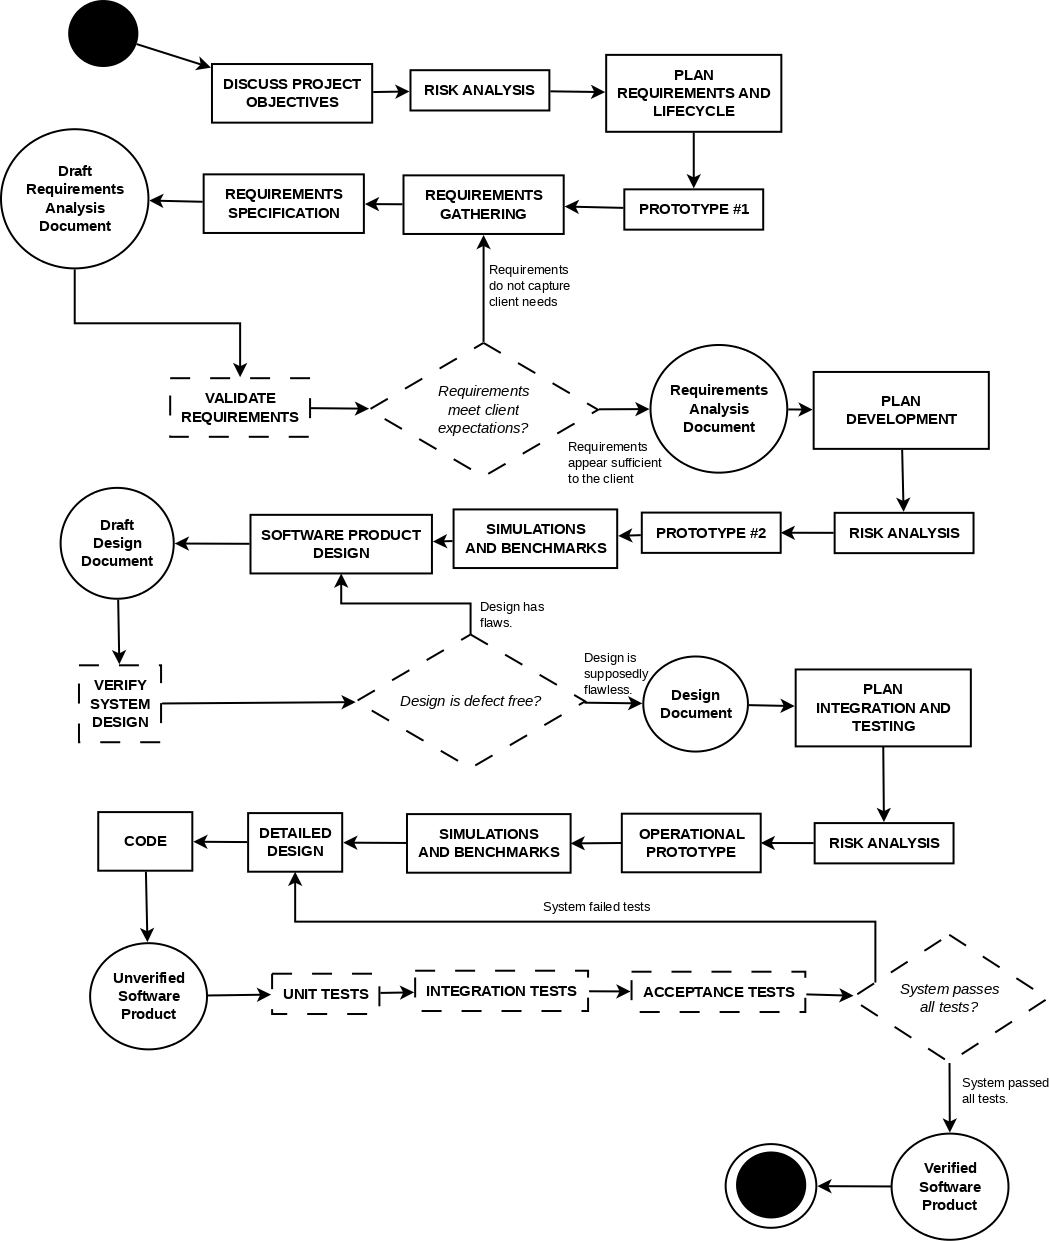
\includegraphics[scale=0.3]{media/Spiral}
	\caption{Barry Boehm's spiral model. We note that it is quite similar to Figure
		\ref{waterfallRoyceThree}.}
	\label{Spiral}
\end{figure}

In reality, this model is actually the SDLC, with more specifications, more risk analysis, and
in \cite{Boehm:1986:SMS:12944.12948} it is rolled up in a spiralling shape.
This does not change that it is really the SDLC waterfall model.
Furthermore, it is unclear in the initial paper what verification is, or where the process should go
back to when a verification point fails.
This is a weakness of the Spiral model, and the Waterfall models as well, though Boehm is more
explicit as to where backtracking should lead to when a defect is uncovered.\\
\\
The spiral model does not represent a significant shift in industry mindset and indeed, we note that
it still ascribes to the ``single stage, verifiy that everything is correct, move onto next stage"
mindset that early industry had.

\subsection{V-Model}

We note that the V-Model is perhaps one of the last of the Waterfall-esque models.
It is introduced by Fosberg et. al in \cite{forsberg1995relationship}.
Again, we note its roots in systems and ``traditional" engineering, where a stage-by-stage based
approach is taken.
Its main difference is perhaps the large amount of preparation and planning to construct plans for
verification.
These plans are constructed before project implementation, and the explicit highlighting of this
construction distinguishes SLDC from the V-model.
We show the V-Model within our notation in Figure \ref{VModel}.

\begin{figure}[ht!]
	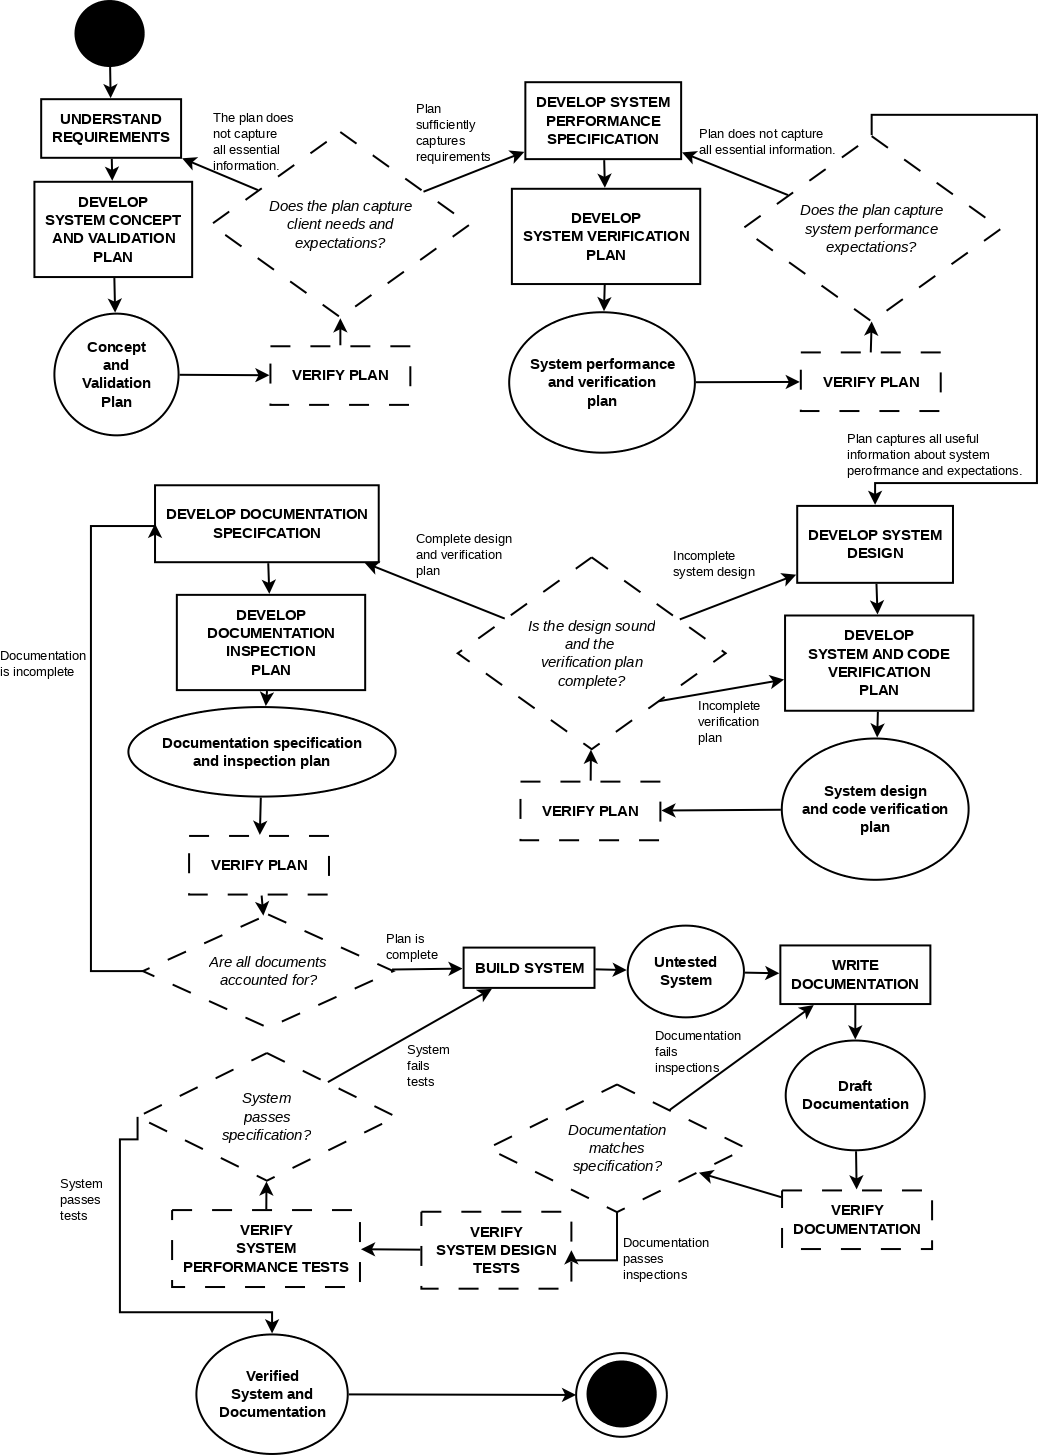
\includegraphics[scale=0.3]{media/VModel}
	\caption{The V-Model, as represented within our notation. Due to its many verification construction stages it is quite an extensive
		model within our notation. One might comment that it is a weakness of our notation that some
			models have become extremely large.}
	\label{VModel}
\end{figure}

\subsection{Rapid Prototyping}
Rapid prototyping, as was specified in \cite{Alavi:1984:APA:358080.358095}, is a process
specifically concerned with requirements gathering.
It constructs small prototypes that are mockups of the final system to assist in understanding a
client's requirements.
As a result, we will make two simplifications for our modelling of the rapid prototyping process.
\begin{enumerate}
	\item the process only changes requirements gathering, and other processes remain the same
	\item we need only model requirements gathering process, up to the generation of a requirements
	analysis document to show how rapid prototyping works
\end{enumerate}

Based on these assumptions, we show Rapid Prototyping in our own notation --- see Figure
\ref{RapidProto}. We note that this methodology would be ineffective in the case that building a prototype would be very
inexpensive or a user might not have much interaction with the system.

\begin{figure}[ht!]
	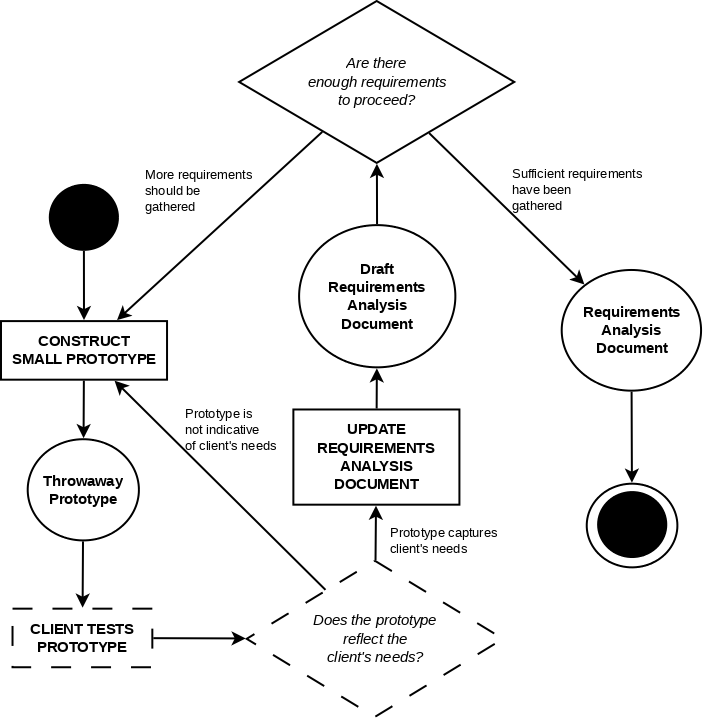
\includegraphics[scale=0.4]{media/RapidPrototyping}
	\caption{Rapid prototyping is shown above, only being used in the requirements gathering stage.
		This is also known as ``throwaway prototyping", due to the prototype being used onl in
			requirements gathering, but not in production code.}
	\label{RapidProto}
\end{figure}

\subsection{Evolutionary}
\subsection{Incremental}

\subsection{Extreme Programming}

\subsection{Crystal Clear}

\subsection{Kanban}

\subsection{Scrum}
The Scrum model was first introduced by Takeuchi and Nonaka in \cite{takeuchi1986new}.
This is a much more agile-like process, without as many sequential steps and many more iterative
loops and decision points.
It eschews documentation and analysis for coding and continuous design.
This would be appropriate for user-facing software that an engineer or development team is already
familiar in coding or working with.
We show a representation of the Scrum process in our own notation in Figure \ref{ScrumFig}.

\begin{figure}[ht!]
	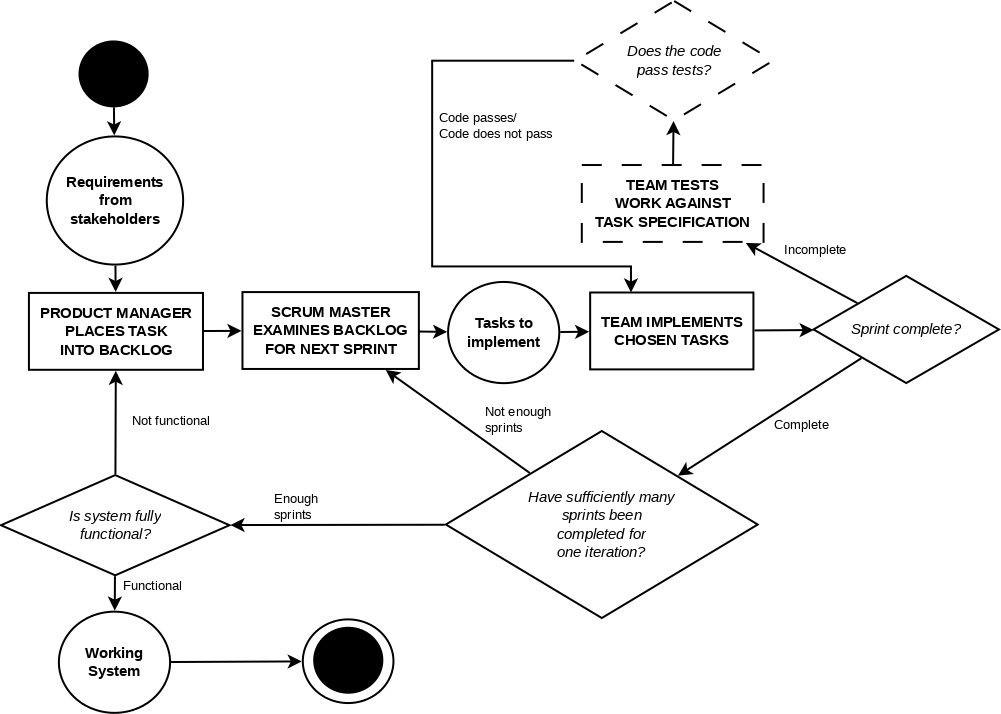
\includegraphics[scale=0.3]{media/Scrum}
	\caption{Scrum is a development model for software, and here we can see the feedback and
		simplified, easy-to-understand and responsive process that Scrum employs.}
	\label{ScrumFig}
\end{figure}
